\documentclass[11pt,a4paper]{article}

\newcommand{\tumsoTime}{13:00 น. - 16:00 น.}
\newcommand{\tumsoRound}{2}

\usepackage{../tumso}

\begin{document}

\begin{problem}{Olympiad in AI}{standard input}{standard output}{1 second}{128 megabytes}{0}

ทุกวันนี้กระแส Artificial Intelligence (AI) มาแรงเกิน จนทำให้สาย Pure Algorithm อย่างเด็กคอมพิวเตอร์โอลิมปิกอยู่ยาก ในอนาคตการแข่งขันคอมพิวเตอร์โอลิมปิกอาจจะให้นักเรียนแข่งออกแบบระบบหุ่นยนต์อะไรสักอย่างก็เป็นได้

ลองคิดภาพตามสิ สมมุติว่าการแข่งขันคอมพิวเตอร์โอลิมปิกครั้งที่ $14!$ มีโจทย์คือ ให้นักเรียนที่เข้าแข่งขันทั้งหมด $N$ คนทำระบบรถยนต์อัตโนมัติวิ่งแข่งกัน ณ สนามแข่งรถแห่งหนึ่งซึ่งมีความยาว $M$ เมตร รถใครเข้าเส้นชัยก่อนก็ได้เหรียญทองไป รถใครเข้าช้าหน่อยก็หมดสิทธิ์เข้าค่าย สสวท.

นี่เป็นการแข่งรถ แน่นอนว่าสนามจะต้องมีลู่วิ่งครบทั้งหมด $N$ ลู่วิ่ง ถ้าจะมองว่าสนามเป็นตารางขนาด $N$ แถว $M$ คอลัมน์ก็ไม่ผิด รถของนักเรียนคนที่ $i$ ($1 \leq i \leq N$) จะออกสตาร์ท ณ แถวที่ $i$ คอลัมน์ที่ $0$ (นอกตาราง) แล้วรถจะต้องวิ่งไปเรื่อย ๆ จนกว่าจะถึงแถวที่ $i$ คอลัมน์ที่ $M+1$

ถึงอย่างไรก็ตาม สนามที่นี่ก็ไม่ได้ดีมากนัก บางช่องขรุขระ รถก็ต้องใช้เวลาวิ่งนาน บางช่องเรียบหน่อยรถก็วิ่งได้เร็ว เอาเป็นว่าถ้ารถจะวิ่งผ่านแถวที่ $i$ คอลัมน์ที่ $j$ ($1 \leq i \leq N$, $1 \leq j \leq M$) จะต้องใช้เวลาวิ่ง $T_{ij}$ โชคดีที่การแข่งขันคอมพิวเตอร์โอลิมปิกครั้งที่ $14!$ ไม่มีกฎห้ามรถวิ่งในลู่วิ่งของคนอื่น ดังนั้น รถแต่ละคันสามารถตีเนียนวิ่งเลนอื่นก็ได้ ถึงอย่างไรก็ตาม จะต้องออกสตาร์ทและเข้าเส้นชัย ณ จุดที่กำหนดไว้เท่านั้น

เนื่องจากรถวิ่งเร็วมากอยู่แล้ว ถ้ารถอยู่ที่แถวที่ $i$ คอลัมน์ที่ $j$ รถสามารถเคลื่อนที่ไปยังคอลัมน์ที่ $j+1$ เท่านั้น เคลื่อนที่ย้อนกลับหรือเลี้ยว 90 องศาไม่ได้ แต่รถสามารถเลือกเส้นทางวิ่งได้สามแบบคือ วิ่งตรงต่อไปยังแถวที่ $i$ วิ่งขึ้นไปยังแถวที่ $i-1$ หรือวิ่งลงไปยังแถวที่ $i+1$ (ถ้าเลี้ยวขึ้นหรือลง ห้ามออกนอกตาราง) รถอาจจะวิ่งอยู่บนช่องเดียวกันก็ได้ เพราะในการแข่งรถ รถวิ่งเบียดกันก็ถือว่าปกติ

\begin{center}
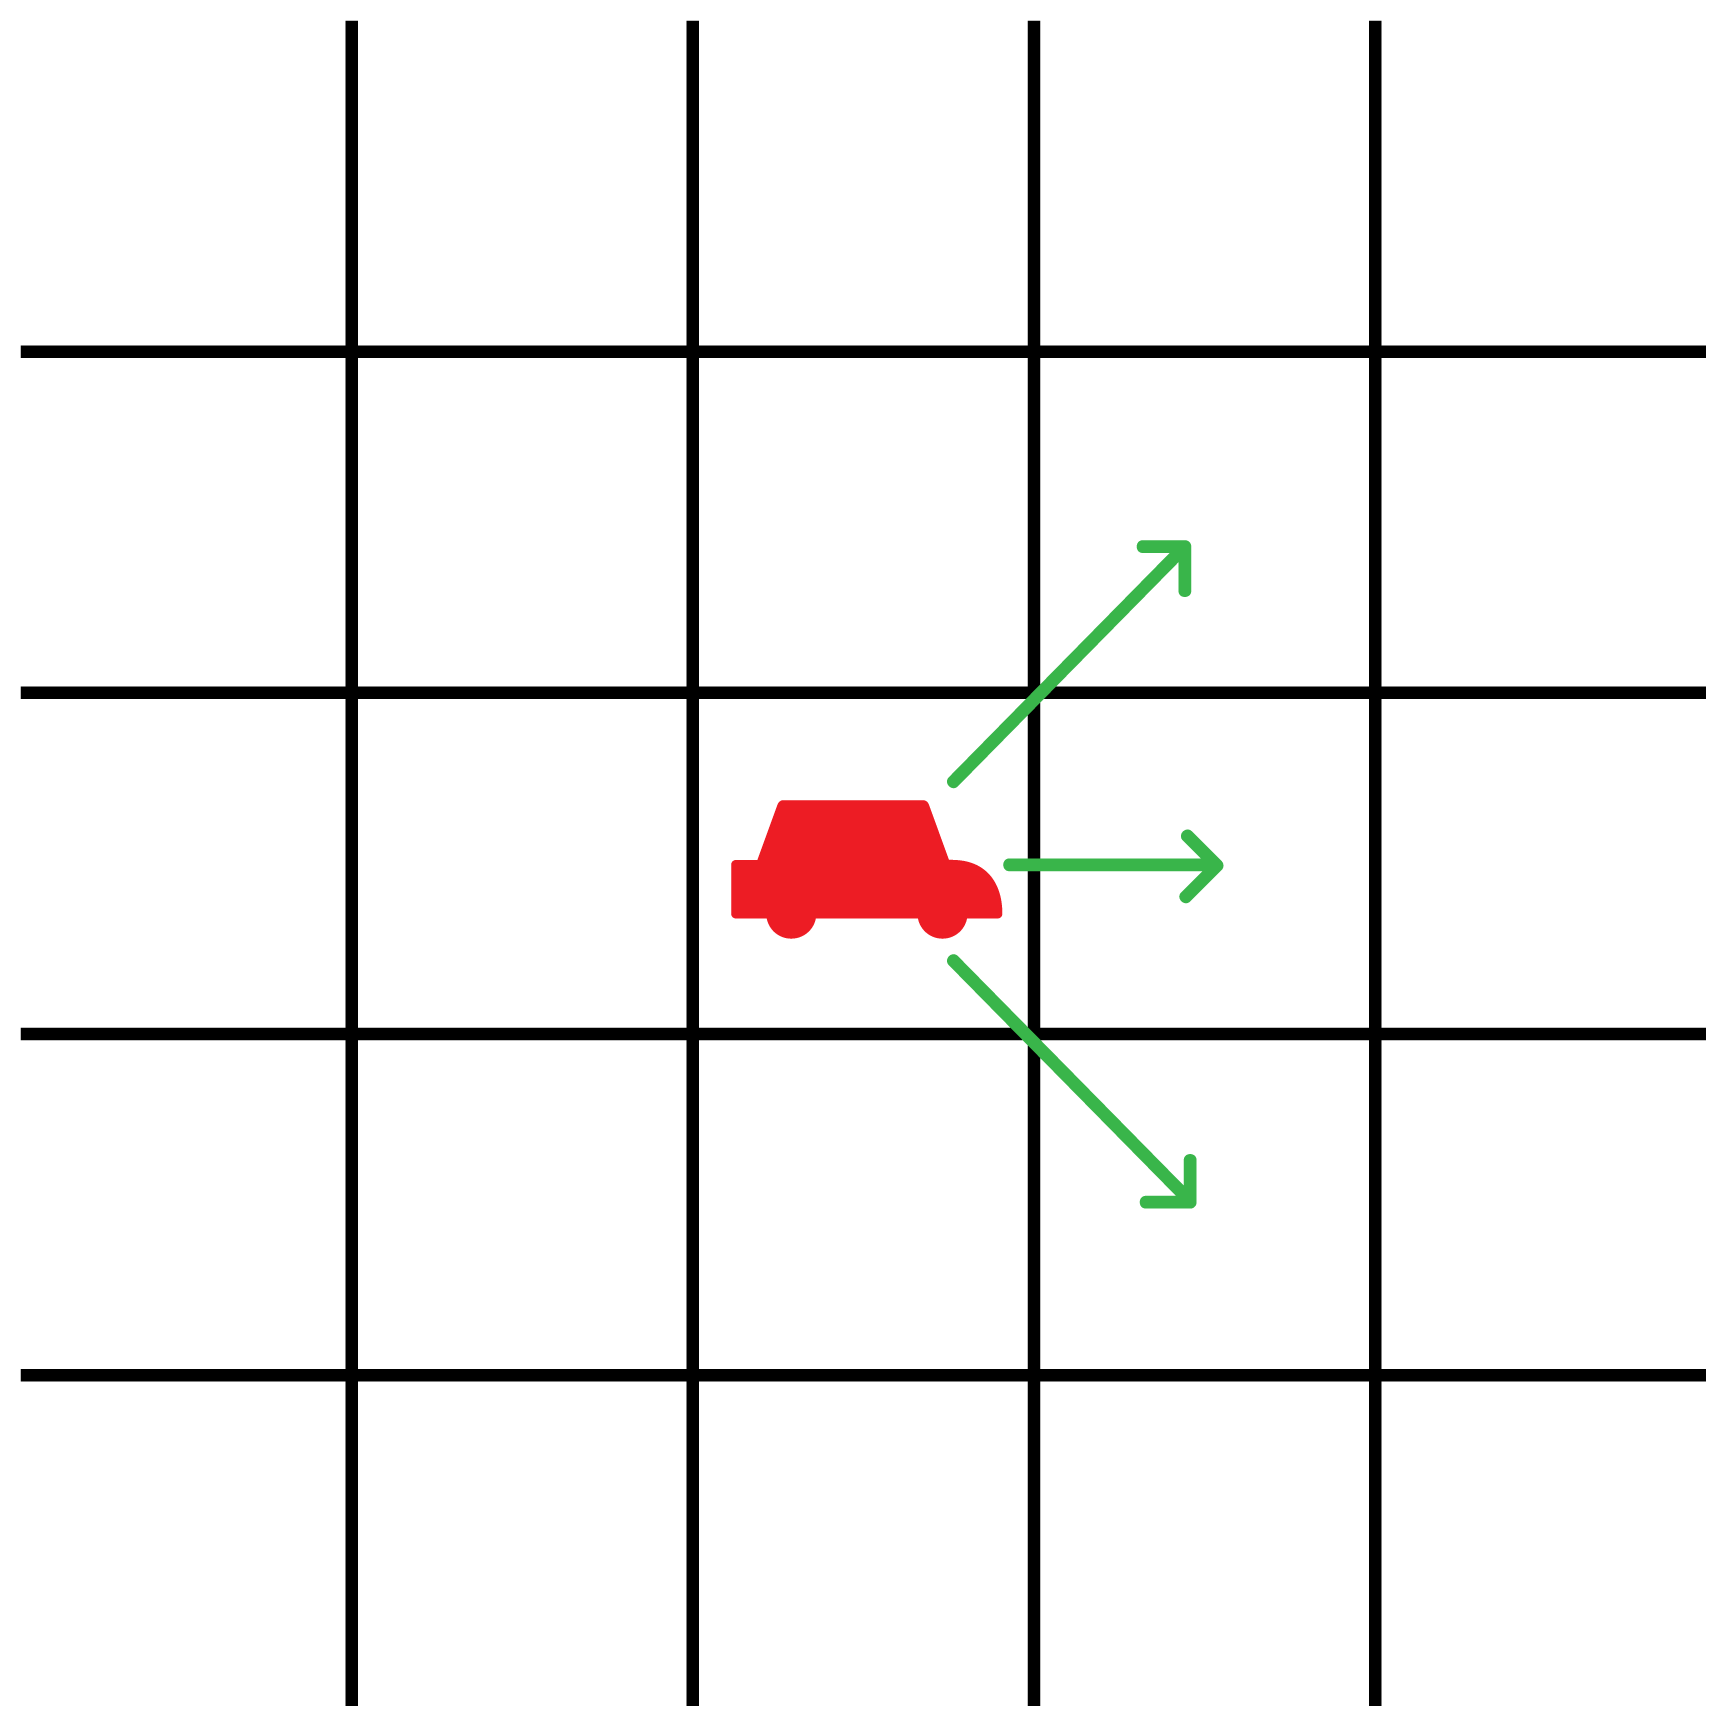
\includegraphics[width=5cm]{car.png}
\end{center}

เราจะกำหนดตารางดังกล่าวมาให้ หน้าที่ของคุณคือหาว่า ถ้าระบบรถยนต์อัตโนมัติของนักเรียนแต่ละคนเลือกเส้นทางที่ดีที่สุด รถแต่ละคันจะใช้เวลาวิ่งเท่าไหร่ก่อนจะถึงเส้นชัย

\InputFile
ข้อมูลนำเข้ามีทั้งหมด $N+1$ บรรทัด

บรรทัดแรก ประกอบด้วยจำนวนเต็มบวก $N$ และ $M$ ($1 \leq N, M \leq 1000$)

บรรทัดที่ $1+i$ ($1 \leq i \leq N$) ประกอบด้วยจำนวนเต็มบวก $T_{ij}$ สำหรับ $1 \leq j \leq M$ ($1 \leq T_{ij} \leq 10^5$)

\OutputFile
ให้ตอบทั้งหมด $N$ บรรทัด ในบรรทัดที่ $i$ ให้ตอบเวลาที่น้อยที่สุดที่รถคันที่ $i$ ต้องใช้เพื่อวิ่งจากจุดเริ่มต้นเข้าเส้นชัย

\Scoring
ชุดทดสอบจะถูกแบ่งเป็น 3 ชุด จะได้คะแนนในแต่ละชุดก็ต่อเมื่อโปรแกรมให้ผลลัพธ์ถูกต้องในชุดทดสอบย่อยทั้งหมด

\begin{description}

\item[ชุดที่ 1 (0 คะแนน)] จะมี $1 \leq N, M \leq 50$

\item[ชุดที่ 2 (0 คะแนน)] จะมี $1 \leq N, M \leq 300$

\item[ชุดที่ 3 (0 คะแนน)] ไม่มีเงื่อนไขเพิ่มเติมนอกเหนือจากที่ระบุไว้ในโจทย์

\end{description}

\Example

\begin{example}
\exmp{4 5
1 2 9 3 5
1 2 4 6 5
9 7 8 3 7
1 3 5 1 1
}{15
15
11
11
}%
\end{example}

\Note
\begin{center}
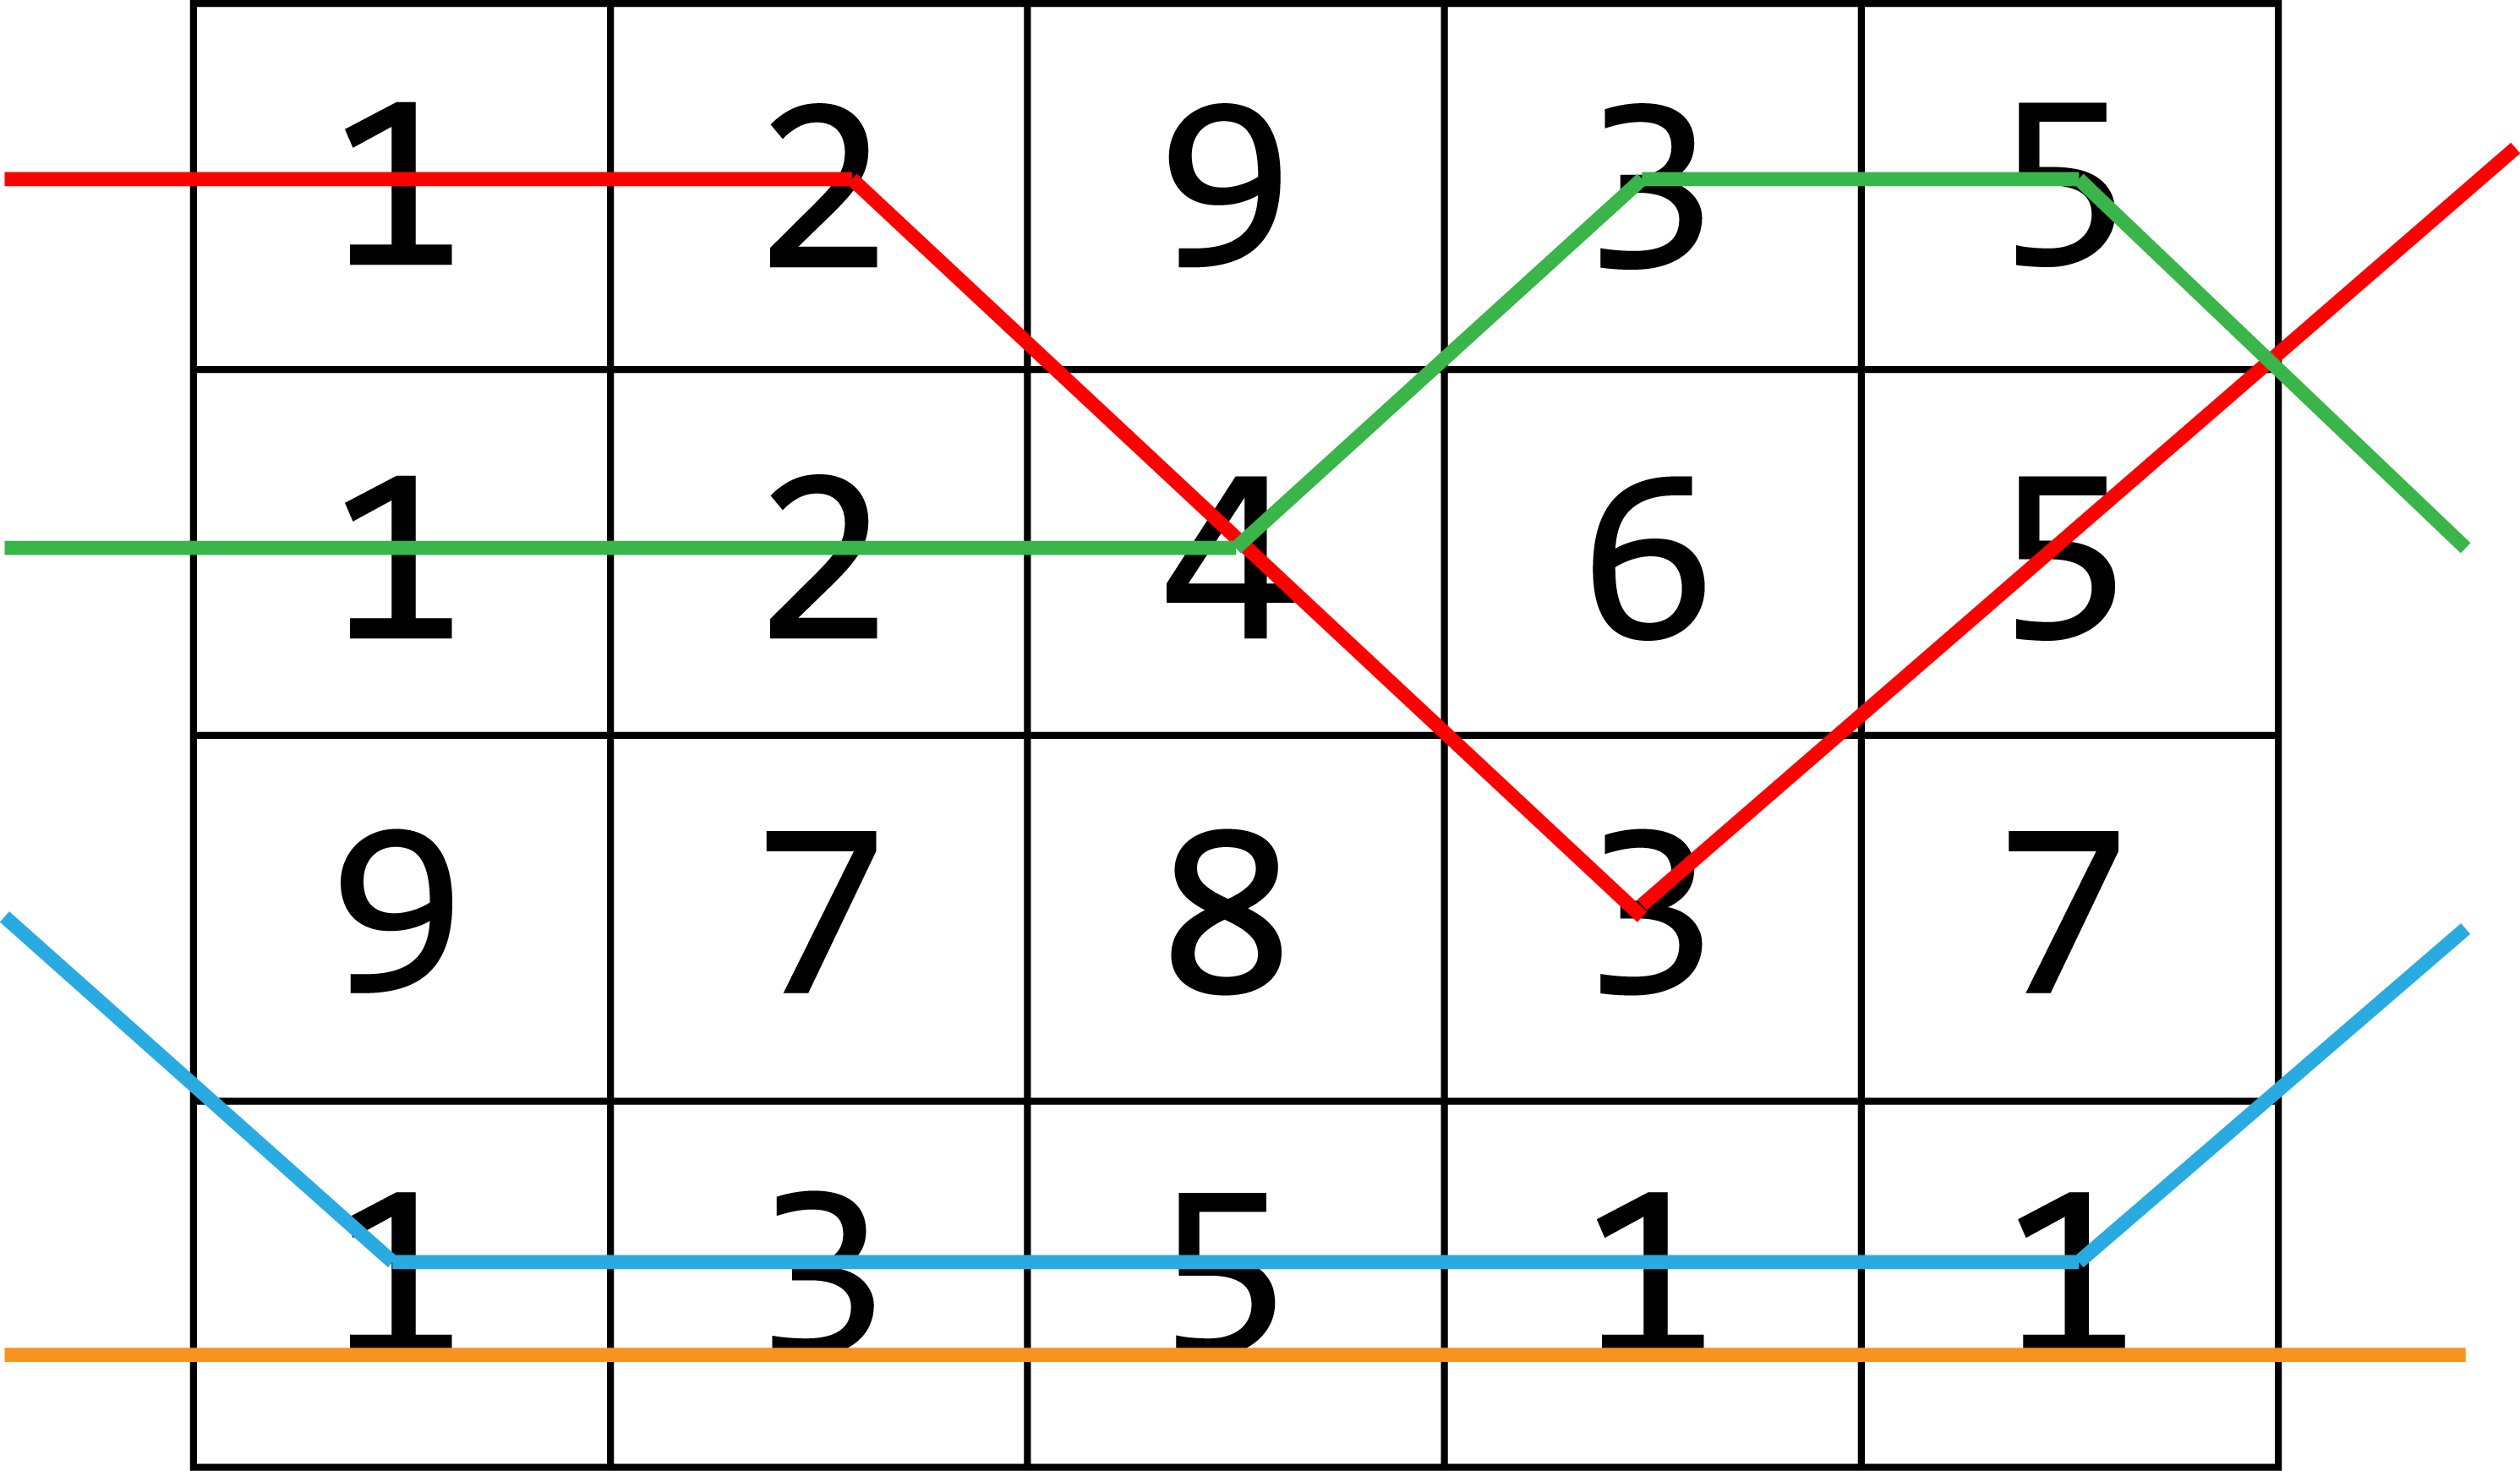
\includegraphics[width=8cm, height=5cm]{numtable.png}
\end{center}


\end{problem}

\end{document}